\scanpage{122}
\mspage{121}


field and if one restricts oneself to finitely generated modules over $k$, one is in the conditions of 6), and one finds the algebraic group $\underline{G}_m$ over $k$. Moreover even without a condition on $k$ and without restricting oneself to finitely generated modules, one recovers $C$ with all these structures through the representations of $\underline{G}_m$\handwritten{\unsure{!|/}}

Let us keep $\unsure{\otimes|\Omega}$, $\handwritten{\phi}$ (and $\underline{1},u,v$) as above, but change $\handwritten{\unsure{\psi|\mu}}$ \deleted{to \rlap{\unsure{l}}$\handwritten{\unsure{\phi|\psi}}$e}, by \deleted{tui} using the Koszul rule. This\inserted{\handwritten{new}\handwritten{\begin{tikzpicture}[x=.45cm,y=.45cm,baseline=-.2ex]\draw (0,-.32) .. controls (.05,-.04) and (.16,.06) .. (.38,.08)--(1.8,.06) .. controls (2.02,.08) and (2.14,.22) .. (2.16,.45);\end{tikzpicture}}} choice of $\handwritten{\unsure{\mu|\psi}}$ is forced in certain questions. For example suppose $k$ a field, \deleted{of characteristic zero,} let $V$ be the category of compact topological spaces, with the functor $\otimes$ given b\unsure{y} Cartesian product, and the obvious datum of associativity and commutativity (this t\deleted{a}ime one really has no choice !); there is\deleted{\unsure{u|n}} a unit, \unsure{that is to} \unsure{\rlap{a}s|$\mathbb{s}$}\unsure{\rlap{s}a|$\mathbb{a}$}y th\deleted{es}e one-point space\deleted{s}. Let us consider the cohomological functor $X\handwritten{\mapsto}H^{\handwritten{\bullet}}(X,k)$ on $V^{\unsure{o|0}}$, using Künneth one finds an isomorphism $c$ of compatibility with the $\otimes$\inserted{from $V^o$ to $C$\handwritten{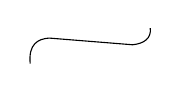
\begin{tikzpicture}[x=.5cm,y=.5cm,baseline=-.2ex]\draw (0,-.45) .. controls (-.05,.05) and (.2,.18) .. (.48,.2)--(2.6,.03) .. controls (2.9,.06) and (3.08,.2) .. (3.05,.45);\end{tikzpicture}}}. The latter is compatible with the structures a),b),c) \uline{on condition} of choosing $\handwritten{\mu}$ in $C$ by the Koko rule\rlap{\raisebox{.65ex}{\deleted{\unsure{f}}}}\handwritten{!}

To prove that when one takes $C$\makebox[0pt][c]{\handwritten{\begin{tikzpicture}[x=.32cm,y=.32cm,baseline=0pt]\draw (0,-.65) .. controls (-.06,.1) and (.03,.4) .. (0,.7);\end{tikzpicture}}}as above in the Koko manner, there\deleted{is} is no fibre functor on $C$ over any extension $K$ of $k$ (even when\deleted{s} restricting oneself to vector spaces of finite di\rlap{e}m\rlap{m}ension) !



\margin{???}
\margin{\figure{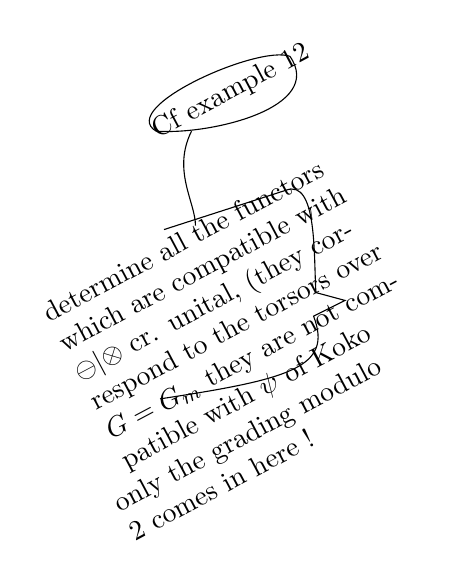
\begin{tikzpicture}[baseline]
\node[rotate=28] at (1.05,4.9) {\handwritten{Cf example 12}};
\draw (.1,4.4) .. controls (-.4,4.7) and (1.4,5.5) .. (1.8,5.35) .. controls (2.25,4.7) and (.8,4.35) .. (.1,4.4);
\draw (.55,4.4) .. controls (.3,3.9) and (.6,3.5) .. (.6,3.2);
\draw (.2,3.15)--(1.75,3.65) .. controls (2.15,3.8) and (2.1,2.8) .. (2.13,2.35)--(2.5,2.25)--(2.1,2.05) .. controls (2.35,1.4) and (1.8,1.25) .. (.15,1.0);
\node[rotate=28,align=left,text width=4.2cm] at (1.05,2.1) {\handwritten{determine all the functors which are compatible with $\unsure{\ominus|\otimes}$ cr. unital, \unsure{(}they correspond to the torsors over $G=G_m$ \uline{they are not compatible with $\psi$ \unsure{of} Koko}}};
\node[rotate=28,align=left,text width=3.9cm] at (1.4,.4) {\handwritten{only the grading modulo $2$ comes in here !}};
\end{tikzpicture}}}

8) To remedy this drawback, it is appropriate\deleted{when one goes into a category with $\otimes$ the category of} t\deleted{e}o study systematically the $\otimes$-functors compatib\rlap{e}l\rlap{s}e with a)b)c) with values in a category\inserted{of \unsure{graded|graded} modules\handwritten{\begin{tikzpicture}[x=.48cm,y=.48cm,baseline=-.2ex]\draw (0,-.45) .. controls (-.08,.05) and (.16,.16) .. (.45,.17)--(2.7,.15) .. controls (2.93,.15) and (3.08,.19) .. (3.05,.4);\end{tikzpicture}}} $\unsure{\rlap{\(X\)}C|\mathbb{C}}$ as above: these are \rlap{d}\handwritten{t}he\handwritten{``}\uline{twisted fibre functors}\handwritten{''}. In particular, if $C$ is as at the beginning of 6) (no $\otimes$ yet), suppose that the functor $F$ factors (in a given way) through graded modules, i.e. that one has a functor compatible with the forgetful functors $C\handwritten{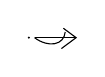
\begin{tikzpicture}[x=.6cm,y=.6cm,baseline=-.1ex]\fill (-.12,0) circle (.025);\draw (0,0)--(.85,0);\draw (0,0) .. controls (.3,-.22) and (.62,-.16) .. (.65,.12);\draw (.61,.2)--(.88,0)--(.57,-.23);\end{tikzpicture}}\mathrm{Gradf}(k)\unsure{\begin{tikzpicture}[x=1em,y=1em,baseline=-.1ex]\draw[line width=.6pt] (0,.32)--(.8,.32);\draw[line width=.8pt] (0,.08)--(.8,.08);\draw[line width=1.2pt] (.33,.08)--(.34,-.08);\draw[line width=.8pt] (.54,.08)--(.55,-.06);\end{tikzpicture}|=|\equiv}\mathbb{D}^{\unsure{\mathbb{X}|X}}$. This corresponds to a homomorphism of coalgebras from $A$ to $k\handwritten{[}T,T^{-1}\handwritten{]}$; where to the datum of elements $\handwritten{\pi}_i$ of $U$ (the projections onto the homogeneous components) satisfying the usual conditions \deleted{$\unsure{\handwritten{\pi}}_i^2=0,\unsure{\handwritten{\pi}_i|i}$}
